% Document class / Dokumentenklasse:
\documentclass{LNTthesis}
% Parameters of the LNTthesis class:
% DIV12       = document layout: DIV factor = 12 (larger number creates larger pages)
% BCOR12mm    = binding correction: 12mm
% headsepline = separate page head by a line
% twoside     = twosided document
% 11pt        = font size 11 point
% openright   = start new chapters only on right pages (odd numbered pages)
% more information: http://tug.ctan.org/tex-archive/macros/latex/contrib/koma-script/scrguien.pdf

% Packages used in LNTthesis class:
% package[english]{babel}   % english language / Englische Sprache
% package{LNTthesis}        % LNT specific definitions / LNT spezifische Definitionen
% package{graphicx}         % for using eps images / Einbinden von EPS Grafiken
% package{verbatim}         % for quickly commenting out large parts of your text / Um viel Text schnell auskommentieren zu koennen
% package{amssymb}          % additional math symbols / Zusaetzliche mathematische Symbole
% package{amsmath}          % additional math commands / Zusaetzliche mathematische Befehle
% package{amsxtra}          % even more math symbols / Noch mehr mathematische Symbole
% package{amsthm}           % theorem environment etc / Theorem Umgebung usw
% more information on amsmath: http://www.ctan.org/get/macros/latex/required/amslatex/math/amsldoc.pdf

% package{psfrag}           % psfrag: http://www.ctan.org/get/macros/latex/contrib/psfrag/pfgguide.pdf
% package{subfigure}        % enable subfigures / Ermoeglicht Subfigures (mehrere Figures neben/untereinander)

% !! PLEASE READ THE LATEX HELP IF YOU HAVE ANY QUESTIONS !!
% http://tobi.oetiker.ch/lshort/lshort.pdf


% Macros:
    \newcommand{\eq}[1]{Equation (\ref{#1})}        % \eg{eq:golomb}  --> Equation (2.15)
    \newcommand{\eref}[1]{(\ref{#1})}               % \eg{eq:golomb}  --> (2.15)
    \newcommand{\fig}[1]{Figure \ref{#1}}           % \fig{fig:golomb}--> Figure 2.15
    \newcommand{\tab}[1]{Table \ref{#1}}            % \tab{tab:lala}  --> Table 2.15
    \newtheorem{prop}{Proposition}

% Abbreviations
    \newcommand{\equivalent}{\triangleq}
    \newcommand{\given}{\:\!\vert\:\!}


% ########################################
% Yadhu defined
% #########################################
\newcommand\TODO[1]{\textcolor{red}{#1}}

\newcommand\NOTE[1]{\textcolor{blue}{#1}}

\DeclarePairedDelimiter\ceil{\lceil}{\rceil}
\DeclarePairedDelimiter\floor{\lfloor}{\rfloor}

\newenvironment{code}{\captionsetup{type=listing}}{}
\SetupFloatingEnvironment{listing}{name=\textbf{Listing}}


% Document:
\begin{document}

% ###################################
% Title page / Titelseite
% ###################################
\LNTtitle{Master's Thesis}          % Thesis type / Art der Arbeit (Master's Thesis, Diplomarbeit)
    {Polar FEC chain development in software for 5G}                  % Thesis title / Titel der Arbeit
    {Yadhunandana Rajathadripura Kumaraiah}                  % Your name / Name des Diplomanden
    {Dr. Moritz Harteneck, Alexander Heinz, Rohde \& Schwarz \newline
 	 Fabian Steiner M.Sc,
 	 Peihong Yuan M.Sc}                % Advisor / Betreuer
    {M\"unchen, November 2018}          % Munich, Date / Muenchen, Datum
    {Yadhunandana Rajathadripura Kumaraiah\\                 % Your Address / Anschrift des Diplomanden
    Schr\"ofelhofstra\ss e 14 WG 02/02\\
    81375 M\"unchen\\
    yadhu.kumaraiah@tum.de}

\LNTrecht{Yadhunandana Rajathadripura Kumaraiah}             % Your name / Name des Studenten
    {M\"unchen, 12.09.2018}         % Munich, Date / Muenchen, Datum

\cleardoubleemptypage   % start new double page / neue Doppelseite

% ########################################
% Table of Contents / Inhaltsverzeichnis
% ########################################

% roman page numbering, starting with page number 1 / roemische Seitennummerierung beginnend mit Seite 1
    \setcounter{page}{1}
    \pagenumbering{roman}

        \tableofcontents    % Table of contents / Inhaltsverzeichnis
        \listoffigures      % List of figures / Abbildungsverzeichnis
        \listoftables       % List of tables / Tabellenverzeichnis
        \cleardoubleemptypage   % start new double page / neue Doppelseite

% ########################################
% Chapters / Kapitel:
% ########################################

% arabic page numbering, starting with page number 1 / arabische Seitennummerierung beginnend mit Seite 1
    \setcounter{page}{1}
    \pagenumbering{arabic}

        %%%%%%%%%%%%%%%%%%%
\chapter*{Abstract}
%%%%%%%%%%%%%%%%%%%
Software implementation of error correction and signal processing applications on general purpose processors has gained interest in recent times. Mainly due to latest technological developments in general purpose computing world. Implementations in software have an inherent advantage not being tied to one specific hardware architecture. They require much less development and maintenance effort compared to hardware implementations. For the device manufacturer software implementation provides platform flexibility in addition to reducing the cost of product. \newline

In this thesis, we study the feasibility of developing complete polar FEC chain of $5^{th}$ generation cellular mobile communication standard in software. Specifically on general purpose processors. Thesis work attempts to achieve stringent latency requirements through software, algorithmic and platform specific optimizations. Many algorithms in FEC chain are optimized for hardware implementations. Direct implementation of these algorithms in software results in poor performance. To obtain best performance on general purpose processors these algorithms are modified or reformulated to suit software implementation. Initially both encoding and decoding FEC chain are implemented functionally without any algorithm reformulation or optimization. Code profiling is performed on this naive implementation to identify the significant latency contributors. We split algorithms of significant latency contributing components into primitive operations. These primitive operations are mapped to specialized functional units of general purpose processor to achieve best performance. \newline

We concentrate on polar encoding and decoding FEC chain which are used to transmit and receive control information. Latency contributing components are identified. Algorithms of those components are reformulated to avoid or to reduce latency contributing operations. Major latency contributors in encoding FEC chain are Cyclic redundancy check (CRC) calculation, polar code construction and  polar encoding. In decoding FEC chain  subblock deinterleaver, polar decoder, parity bit extraction and CRC calculation. Algorithms of these components are reformulated to suit software requirements and implemented using efficient \emph{vector processing instruction sets}. Algorithms are modified to reduce complexity and lookup tables are used to avoid complex computations. Other optimizations include function unrolling, avoiding superfluous copy operations, hints to compiler for better instruction scheduling and block wise copying et cetera. At the end of both encoding and decoding chapter latency comparisons between naive and optimized implementations are presented. In decoding FEC chain chapter, latencies of decoder of this work and state of the art decoder are compared.     % Include abstract / Einbinden von Kurzfassung und Abstract
        %%%%%%%%%%%%%%%%%%%%%%%%%%%%%%%%%%%%%%%%%%%%%%%
\chapter{Introduction and Motivation} \label{chap:introduction}
%%%%%%%%%%%%%%%%%%%%%%%%%%%%%%%%%%%%%%%%%%%%%%%

\section{Era of Computing and Wireless Communication}
Ability to perform computations has evolved tremendously from the day first computer was invented by charles babbage in the 19th century. By the end 19th century another important event occurred, in 1897 an italian inventor and engineer Guglielmo Marconi demonstrated radio's ability to maintain continuous contact with ships in english channel. Major breakthrough happened in the development of computers and wireless systems in 1948, when scientists at the Bell achieved ground breaking results. Claude E.~Shannon published his paper \emph{A mathematical theory of communication} and John Bardeen, Walter Brattain and William Shockley announced the invention of the \emph{transistor effect}. These two landmark events paved way for the widespread adoption of computers and wireless communication systems in numerous applications. Since then telecommunication industry has grown manifold fueled by the advancements in RF and transistor fabrication techniques, miniaturization and Very Large Scale Integration. These technological advances made computing devices smaller, cheaper and more reliable. Recent advances in wireless communication have allowed not only short distance communication such as cellular communication even billions of kilometers distance deep space communication. \newline

Today computing devices and wireless systems have become integral parts of our society. They allow communication between people even from remote areas. Invention of Internet has enabled people to have access to world of information in their fingertips. Till recently, wireless devices were primarily used for information exchange between people. Today wireless applications are entering new avenues such as industrial automation, telemedicine, Autonomous driving. These applications demand ultra-reliability and ultra-low-latency. Latest mobile communication standard 5G took a giant step towards providing service for such mission critical applications. 5G has adopted several techniques to service stringent latency requirements. To name few, different OFDM numerologies, flexible frame structure et cetera. Traditionally to achieve stringent latency requirements wireless communication stacks are implemented in hardware, specifically in FPGAs/ASICs. Hardware implementations make use of implicit hardware-concurrency. However hardware implementations come with inherent non-flexibility, huge cost and high development time. Due to latest technological advancements in general-purpose computing, Modern processors come with a tremendous computation power. It is up to software engineer to efficiently harness this computational power. Modern processors come with special computing units to cater to specific application domains, namely vector processing units for signal processing applications. To achieve stringent latency requirements, it is very important that a software designer makes use of these additional processing elements and available optimization techniques.

%Traditionally FEC chains are developed in hardware i.e FPGA’s or ASIC’s to achieve low latency and high throughput.
%Development in FPGA/hardware requires more time and costly.
%With recent advances in General Purpose Processors it is possible to achieve required latency and throughput with software implementations without custom hardware.
%Software implementations are flexible and easy to maintain compared hardware implementations.
%
%However algorithms need to be adopted/optimized to efficiently implement in software.
%
%Recent advances in the modern processors such as SIMD units can be utilized to achieve low latency and high throughput.

\section{Polar FEC chain development in software}
Commonly high performance signal processing and error correction applications are implemented in hardware either in FPGAs/ASICs. Hardware implementations allow these applications to achieve low latency and high throughput. Algorithms in these applications are developed targeting hardware implementations. These algorithms implemented in software without any reformulation or modification result in poor performance. Therefore algorithms need to be modified and reformulated to achieve expected performance in software. \newline

Optimizations for hardware such as recursive formulation, reducing look up tables (LUTs) and flip flops are not always relevant in software. Let's try to understand conflicts in the optimizations targeted for hardware and software. Most of the encoder/decoder algorithms are formulated in recursive form. In hardware implementations recursive formulations particularly useful since same design can be replicated multiple times without significant design effort also with no performance compromise. However in software implementations recursive implementation incur significant overhead. Mainly due to large of branchings, stack allocation/deallocation and pipeline flushing. Next optimization in hardware targeted implementations is minimizing the required memory and flip-flops. In contrast general purpose computing world can make use of off-the-shelve available cheap memory but software designer should make reduce cache misses, branch miss predictions. In addition, software implementations should also make sure to avoid expensive operations such as multiplications, division and modulus operations. If not, reformulate them by using inexpensive bitwise operators. \newline

It is clear from above discussed details that algorithms directly implemented in software without modification or reformulation result in poor performance. To achieve best performance in software algorithms must be broken down into smaller operations then should be mapped to specific functional units of modern processors. For example, when huge number of floating point/integer operations involved. These computations must be mapped to specialized vector processing units (SIMD) which are specifically designed perform these operations. Mapping to vector processing units allows data parallelism. If algorithm requires lot of memory accesses, software should make use of special cache prefetching units to hide memory access latency. If huge data must be moved copied based on previous decisions, such operations must be mapped to conditional move instructions and so forth.  Figure \ref{fig:operationMapping} gives visual illustration of mapping operations to specialized processing units/instructions.

\begin{figure}[]
	\centering
	\includegraphics[width=1\textwidth]{./figures/operationMapping.pdf}
	\caption{Mapping FEC chain operations to particular functional units}
	\label{fig:operationMapping}
\end{figure}

This thesis work is a step in that direction. It tries to achieve maximum performance out of modern general purpose processors to satisfy stringent latency requirements. Latest 3GPP standard has adopted polar codes for encoding and decoding control channel information \cite{3gpp.38.212}. Downlink control information (DCI) and Uplink control information (UCI) are transmitted using polar codes. In this work, polar encoding and decoding FEC chain is implemented in software. FEC chain algorithms are reformulated/optimized to suit software implementation. FEC chain functionalities are broken down in to primitive operations and are mapped to specific computational units of general purpose processor. Implementation uses off-the-shelf available AMD EPYC general purpose processor\cite{amdEpyc}. It comes with state-of-the art instruction extensions. These advanced instructions allow mapping different operations in FEC chain implementation to specialized processing units to maximize performance.

Software implementation in this work makes extensive use of vector processing units, cache prefetching, branch prediction and compiler optimizations to achieve low latency. After the implementation each component of FEC chain performance of naive and optimized implementations are presented. At the end of encoding and decoding FEC chain chapters, latency whole FEC chain  is presented. Comparison between functional and optimized implementation is given to understand the importance of software optimizations. In decoding FEC chain chapter performance of implemented decoder is compared with state of the art software decoder implementation \cite{lowLatencySWPolarDec}.

\section*{Organization of the Thesis}
Having described the overall problem and relevant motivation, in Chapter 2 the necessary background to develop polar FEC chain is provided. Including required mathematical understanding of polar codes and fundamentals of modern computer architecture. In Chapter 3, details of the polar encoding FEC chain are presented. Each of components are analyzed for latency contribution. Both algorithmic and software optimizations are employed. At end latency of naive and optimized implementations are compared. In Chapter 4, details of polar decoding FEC chain are presented. Operation of different components in the FEC chain are given in detail. Each operation is optimized by mapping them efficiently specific instructions/processing units. Decoder algorithm optimizations are presented and compared with state of the art software decoder implementations. Finally at end of Chapter 3, latency of the optimized decoding FEC chain is compared with the naive implementation.  % Include introduction / Einbinden des Kapitels Einleitung/Problemstellung
        \chapter{Background} \label{chap:Background}

\setcounter{secnumdepth}{3}
\renewcommand{\thesubsubsection}{\Alph{subsubsection}}

%\titleformat{\subsubsection}
%{\selectfont}{\thesubsubsection}{1em}{}

%Give background about polar codes and their adoption in 5G.

Polar codes were introduced by Ar\i kan in his seminal work \cite{Arikan}. They belong to the class of capacity achieving codes. In the past decade, polar codes have sparked a interest from both academia and industry alike, resulting in significant research work in improving performance. The 5\textsuperscript{th} generation wireless systems (5G) standardization has adopted polar codes for uplink and downlink control information for the enhanced mobile broadband (eMBB). They are also considered as the potential coding schemes for two other frameworks of 5G, namely ultra-reliable-low-latency (URLLC) and massive machine-type communications (mMTC).

Polar codes achieve capacity asymptotically for memoryless channel. Although they are the first theoretically capacity achieving codes with an explicit construction, capacity is approached only asymptotically. Their performance is suboptimal compared to LDPC (Low Density Parity Check Codes) or Turbo codes at short block lengths with \emph{successive cancellation decoding (SCD)}. In \cite{SCL} the authors present an improved version of SCD called \emph{successive cancellation list decoder (SCLD)}.

The construction of polar codes involves the identification of channel reliability values. Information bits are placed in the $ K $ (number of information bits) high reliable bit indices out of $ N $ (block-length) positions and remaining bits are set to zero. These $ N $ bits are passed through a polar encoding circuit to get the encoded bits. Selection is of reliability indices is done based on the code length and channel signal-to-noise ratio. Due to varying code length and channel conditions in 5G systems, a significant effort has been put into identifying the reliable indices which have good error correction performance over different code length and channel conditions.

\section{Background of Polar codes} 
This section introduces the foundations of the polar codes. In particular, about the frozen set design, encoding and decoding. Different decoding algorithms are introduced. Mainly Successive Cancellation (SC) and Improved Successive Cancellation (fast-SSC)\cite{fastPolarDecodersAlgoImpl}. Examples of encoding and decoding with different algorithms are presented for a better understanding.

%\subsection{Polar codes definition} \label{polarCodesDefn}

The mathematical foundations of polar codes lies in the polarization effect of the kernel \cite{Arikan}. $ \utilde{G} = \big[\begin{smallmatrix} 1 & 0 \\ 1 & 1 \end{smallmatrix}$\big] also called Ar\i kan matrix. Polar codes are $(N,K)$ linear block codes of size $N = 2^{n}$ where $n$ being a natural number. $N$ is the block length of the code and $K$ is the number of information bits.  $N$-bit vector $U$ contains $K$ information and $N-K$ frozen bits which are set to known value mostly zeros. These bits are then multiplied with the generator matrix constructed from kronecker power\cite{kronecker} of Arikan kernel matrix.

For example $n=3$, block-length $N$ becomes $8$ hence the generator matrix is \newline

$ \utilde{G}^{\otimes 3} = \begin{bmatrix}
1 & 0 & 0 & 0 & 0 & 0 & 0 & 0\\ 
1 & 1 & 0 & 0 & 0 & 0 & 0 & 0\\ 
1 & 0 & 1 & 0 & 0 & 0 & 0 & 0\\ 
1 & 1 & 1 & 1 & 0 & 0 & 0 & 0\\ 
1 & 0 & 0 & 0 & 1 & 0 & 0 & 0\\ 
1 & 1 & 0 & 0 & 1 & 1 & 0 & 0\\ 
1 & 0 & 1 & 0 & 1 & 0 & 1 & 0\\ 
1 & 1 & 1 & 1 & 1 & 1 & 1 & 1
\end{bmatrix}$ \newline

where $\utilde{G}^{\otimes n}$ denotes the $n^{th}$ Kronecker power of $\utilde{G}$. The encoding process involves the multiplication of $N$-bit vector $U$ consisting of $K$ information bits and $N-K$ frozen bits with $\utilde{G}^{\otimes n}$.

\subsection{Polar code construction} \label{CodeConstruction}
In polar coding, first step is to identify the channel reliability values for a particular block length, this step is also called polar code construction. Basic idea  is to produce a fraction of channels which are either completely noiseless or noisy out of $N$ (block-length) independent copies of given binary discrete memoryless channel. This process of creating extremal channels is called channel polarization. As $N\to\infty$, fraction of noiseless channels approaches the capacity of channel. Estimating reliability indices of channels is carried by considering the Bhattacharyya parameter\cite{Arikan}. Bhattacharyya parameter indicates the reliability of individual channel.
 
For a generic binary-input discrete memoryless channel (B-DMC) which is represented as $W \colon \mathcal{X} \to \mathcal{Y}$ with input alphabet $\mathcal{X}$, output alphabet $\mathcal{Y}$ and transition probabilities given by $W(y|x),x \in \mathcal{X}, y \in \mathcal{Y}$.

Bhattacharyya parameter is given by 
\begin{equation}
	Z(W) \triangleq \sum_{y \in \mathcal{Y}} \sqrt{W(y|0)W(y|1)}
\end{equation}

The Bhattacharyya parameter indicates how unreliable the channel is, It is easy see that $Z(W)$ takes values between $[0,1]$ better the channel smaller is the $Z(W)$. Polarization for $N \to \infty$ creates channels with either $Z(W) \to 0$ or $Z(W) \to 1$.

\begin{figure}[h]
	\centering
%	\includegraphics[width=1\textwidth]{./figures/channel_polarization_plot.pdf}
	\includegraphics[width=1\textwidth]{./figures/channelPolarization1.pdf}
	\caption{Channel polarization example for binary erasure channel with $\epsilon = 0.4$}
	\label{fig:channelPolarizationPlot}
\end{figure}

Figure \ref{fig:channelPolarizationPlot} illustrates channel polarization for different block lengths for binary erasure channel with erasure probability $\epsilon = 0.4$. It can be seen that as block-length increases channels gets polarized to extremal channels (either completely reliable or unreliable).

\subsection{Encoding} \label{polarEncoding}
After $N-K$ frozen bit positions have been found, they are set to zero and information bits are placed in remaining $K$ positions.
%After polar code constructions, Out of $N$ bit positions information bits are placed in the most reliable bit indices position and non reliable bit positions are called frozen bits whose values are set to zero.
This $N$-bit vector $U$ is multiplied with generator matrix obtained by the Kronecker power of Ar \i kan kernel matrix. Multiplying with generator matrix can also be represented as circuit form. Ar\i kan kernel matrix can also be represented in a circuit form as shown in Figure \ref{fig:butterFlyCicuit} also called butter fly circuit.

\begin{figure}[h]
	\centering
	\includegraphics{./figures/ButterFlyCircuit.pdf}
	\caption{Butterfly circuit representing Ar\i kan Kernel matrix}
	\label{fig:butterFlyCicuit}
\end{figure}

For an $n = 3$ told Krokecker product, block length $N$ becomes 8 for such a case encoding circuit looks shown in  Figure ~\ref{fig:encoderCircuit}, which is a repeated application of the butter fly circuit. The read locations are the frozen bit indices which are set to zero, in remaining positions information bits are inserted. Output of the circuit is a code word which is transmitted over the channel. Lets consider an example with $N = 8$ and $K = 4$, rate of this code is $R = K/N = 1/2$. As given in the figure frozen bit indices are ${\{0,1,2,4\}}$ remaining indices contain information bits. Let the information bits, which needs to transmitted be \{1,1,0,0\}. After placing information bits at reliable channel positions the vector $U$ becomes \{0,0,0,1,0,1,0,0\}. It is passed through the polar encoding circuit shown in Figure ~\ref{fig:encoderCircuit}. Result at the output of encoder is \{0,0,1,1,1,1,0,0\}. These encoded bits are then transmitted over the channel.

\begin{figure}[h]
	\centering
	\includegraphics[width=0.8\textwidth]{./figures/EncodingCircuitStagesNew.pdf}
	\caption{Polar encoder in circuit form for $N = 8$}
	\label{fig:encoderCircuit}
\end{figure}

The encoding circuit is nothing but recursive application of the transformation represented by the butterfly circuit shown in the figure ~\ref{fig:butterFlyCicuit}. One butterfly unit can transform two uncorrelated bits $(a,b)$ into two correlated output bits $(a\oplus b,b)$. This corresponds to a polarization into two channels. In the above example the reliability of the $u_{1}$ is increased compared to the $u_{0}$. This operation recursively applied to the whole code word results in the circuit shown in the Figure ~\ref{fig:encoderCircuit}. Code word splits into two parts in stage-3, which again splits into two parts in stage-2 and so on, until one reaches to single source bit $u_{i}$ in stage-1. So the process of polar encoding for $N = 8$ involves three stages of butterfly operations. Generally, for a given code length $N=2^{n}$, the polar encoding consists of stages each with $N/2$ butterfly operations, which results in an encoding complexity of $O(N\log(N))$.

%\TODO{If you find any interesting, useful information for better understanding of the polar encoding, don't hesitate to include here.}

\subsection{Decoding}
As shown in section ~\ref{polarEncoding}, repetitive application of butterfly operation during encoding introduces correlation between the source bits. At the receiver, this is exploited to estimate the transmitted codeword. Utilizing the high correlation between the source bits forms the central idea behind the basic polar decoding algorithm called \emph{successive cancellation (SC)} decoding. This method sequentially decodes each of the bits and takes previously estimated value to account for estimating the next bit. This sequential decoding exploits the correlation between the source bits which as introduced during polar encoding process. Due to the sequential nature of SC decoding, the decoding process has high latency. Improving the basic decoding algorithm has been the topic of researchers in academia and industry. These improvements are mainly directed towards two goals, first reducing decoding latency and second improving the error correction performance. Significant reduction in decoding latency is achieved by \cite{SSC} and \cite{fastSSC}. In these works, instead of decoding sequentially individual bit, special nodes are identified which can be decoded in parallel. Although polar codes are the first theoretically capacity achieving codes with explicit construction, their error correction performance at short block lengths is not comparable with that of LDPC or Turbo codes. This behavior can be better explained by the way decoding is performed. As presented earlier SC algorithm works by sequentially decoding individual bits and using information of previously decoded bits for estimating next bit. The issue with algorithm is if the previously decoded bit is wrong, then there is no way of correcting this bit.

To overcome this problem \cite{SCL} presents a improved version of the SC algorithm called \emph{successive cancellation list} (SCL) Decoding . The basic idea is instead of deciding a value of bit $u_{i}$ it takes both options, this results in two decoding paths for every bit, so to avoid exponential growth of complexity decoding candidates are restricted to $L$ the list size. At the end of decoding, most probable candidate is chosen from list. Performance of polar codes with SCL is still not as good as LDPC or Turbo codes at small and moderate block lengths. Polar code concatenated with CRC as outer code beats the LDPC codes of similar block length \cite{SCL}. SCL algorithm has a better error correction performance than SC, however it comes with a increased complexity and high decoding latency. Due to these reasons, in this work concentrates on fast-SSC algorithm is considered although its error correction performance is inferior compared to SCL. Naive SCL algorithm is implemented, however its optimization is considered for the future work.

\paragraph{\emph{A. Successive Cancellation Decoding (SC)}}  \label{SC}
The recursive SC decoder is basic algorithm presented in \cite{Arikan} for decoding polar codes.  SC decoder is inherently sequential, the estimate of $u_{i}$, $\hat{u_{i}}$ is obtained by using channel observation $y^{N}_{1}$ and all the previously decoded bits $\hat{u}_{1}^{i-1}$. If $u_{i}$ is frozen bit, the decoder assigns $\hat{u_{i}}$ to known value (mostly zero). If $u_{i}$ is an information bit, the decoder waits for all the previous bits to compute the decoding metric.  In the following equations $W_{N}^{(i)}$ is a set of N binary-input synthesized channels with output $(y_{1}^{N},\hat{u_{1}}^{i-1})$ and $ u_{i} $ as input, also represented as $W_{N}^{(i)}:\mathcal{X}\to \mathcal{Y^N} \times \mathcal{X}^{i-1}$, $1 \leq i \leq N$. These channels are synthesized from generic binary-input discrete memoryless channel also written as $W:\mathcal{X}\to \mathcal{Y}$ with input alphabet $\mathcal{X}$, input alphabet $\mathcal{Y}$. Synthesized through channel polarization as presented in \cite{Arikan}.  \newline

Decoding metric can be one of the three different type of metrics shown below:

$\bullet$ log-likelihood ratio (LLR) where

\begin{equation}
L_{N}^{(i)}(y_{1}^{N},\hat{u_{1}}^{i-1}) = \ln{\Bigg(\frac{W_{N}^{(i)}(y_{1}^{N},\hat{u_{1}}^{i-1}|u_{i} = 0)} {W_{N}^{(i)}(y_{1}^{N},\hat{u_{1}^{i-1}}|u_{i} = 1)}\Bigg)};
\end{equation}

$\bullet$ likelihood ratio (LR) where 

\begin{equation}
LR_{N}^{(i)}(y_{1}^{N},\hat{u_{1}}^{i-1}) = \Bigg(\frac{W_{N}^{(i)}(y_{1}^{N},\hat{u_{1}}^{i-1}|u_{i} = 0)} {W_{N}^{(i)}(y_{1}^{N},\hat{u_{1}^{i-1}}|u_{i} = 1)}\Bigg);
\end{equation}

$\bullet$ log-likelihood (LL) where 

\begin{equation}
LL(y_{1}^{N},\hat{u_{1}}^{i-1}) = \Big[\ln\Big(W_{N}^{(i)}(y_{1}^{N},\hat{u_{1}}^{i-1}|u_{i} = 0)\Big), \ln\Big(W_{N}^{(i)}(y_{1}^{N},\hat{u_{1}^{i-1}}|u_{i} = 1)\Big)\Big];
\end{equation}

Decoding metrics computed from LLRs exhibit better numerical stability than those from LRs or LLs, so we have used the LLRs metric throughout this work. There are different ways to view and understand the operation of an SC decoder. In this work, decoding is viewed as message passing algorithm on an binary tree with $\log(N)$ levels. Decoding is performed by traversing a tree from root to leaf node. Process of decoding involves check node (CN), variable node (VN) operations and threshold detection at the leaf node. Decoder receives a LLR value for every bit which needs to be decoded (including both frozen and information bits), hence for a code with block length $N$, SC decoder receives $N$ LLR values. Decoding process estimates the bits $\hat{u}_{i} $  where $i = 1,2...,N$. The decoding tree for $N = 8$ looks as shown in the figure ~\ref{fig:decodingTree}.

\begin{figure}[h]
	\centering
	\includegraphics{./figures/decodingTree.pdf}
	\caption{Decoding tree}
	\label{fig:decodingTree}
\end{figure}

\begin{figure}[h]
	\centering
	\includegraphics{./figures/messagePassingDiaS.pdf}
	\caption{Local Decoder}
	\label{fig:msgPassingDia}
\end{figure}

In a decoding  tree, the messages to left child node are computed with CN and to the right are with VN operation.  Figure ~\ref{fig:msgPassingDia} shows how the messages are exchanged in a local component decoder.

The CN and VN operations in LLR domain are given by following equations:

$\bullet$ Check Node (CN) operation

\begin{equation} \label{cnop}
	\alpha_{v_{l}}[i] = \alpha_{v}[i] + \alpha_{v}[i + N_{v}/2]
\end{equation}

$\bullet$ Variable Node (VN) operation

\begin{equation} \label{vnop}
\alpha_{v_{r}}[i] = \alpha_{v}[i + N_{v}/2] + (1 - 2\beta_{v_{l}}[i]) * \alpha_{v}[i]
\end{equation}

After decoding is done at both right and left child nodes the bits are combined at common parent node. the bit combining operation is given by the following equation.

\begin{equation*} \label{bitCombination}
\beta_{v}[i] = \begin{cases}
				\beta_{v_{l}}[i] \oplus \beta_{v_{r}}[i] & \text{if }i < N_{v}/2 \\
				\beta_{v_{r}}[i]
				\end{cases}
\end{equation*}

In the Figure ~\ref{fig:msgPassingDia} and in equations \eqref{cnop}, \eqref{vnop}  $\alpha_{v}$, $\beta_{v}$ represent intermediate LLR values and estimated bits at the local decoder respectively.

Figure \ref{fig:scDecodingEg} gives an example of SC decoding for the block-length $N=8$ and a number of information bits $K=4$. The 16-bit quantized LLR values are an input to the decoder. In the figure, decoded bits and intermediate $\beta_{v}$ are represented by black font color and computed intermediate $\alpha_{v}$ are indicated by green. Frozen pattern is provided below the leaf nodes. Frozen pattern indicates position of information and frozen bits. One in frozen pattern indicates frozen bit, zero indicates information bit.

\begin{figure}[h]
	\centering
	\includegraphics[width=0.9\textwidth]{./figures/SCDecodingExample1.pdf}
	\caption{SC decoding example}
	\label{fig:scDecodingEg}
\end{figure}

%\TODO{provide an example of decoding with real LLR values for $N = 8$}

\paragraph{\emph{B. Improved Successive Cancellation Decoding (fast-SSC)}\newline}  \label{fastSSC} 
In the basic SC algorithm, decoding is performed sequentially, previously decoded values are used for decoding the present bit. Due to sequential nature of the decoder, decoding latency is high. The works \cite{SSC} and \cite{fastSSC} try to identify special kind of nodes in a decoder tree which can be immediately decoded without traversing till the end of tree. In \cite{SSC}, the authors try to identify the nodes which are associated with all information or frozen bits. These nodes are called rate-one ($R1$) and rate-zero ($R0$) nodes respectively. The $R1$ node can be decoded by taking hard decisions and a polar transform, since there is no extra information which can be gained from traversing the tree. The decoding of $R0$ nodes is not necessary since none of them are information bits, so all the bits are set known value which is known at transmitter and receiver which are mostly set to zero. \par Authors in \cite{fastSSC} extend the idea presented in \cite{SSC} by identifying two additional kinds of special nodes which can be decoded without traversing the tree single parity check ($SPC$) and repetition ($REP$) nodes. Both in \cite{SSC} and \cite{fastSSC}, the node type is identified based on the frozen pattern at the component decoder. For a $SPC$ node, only one frozen bit is present at left most position. For a $REP$ node, frozen pattern contains one information bit at right most position, remaining are frozen bits.

One such example, when frozen indices for $N = 8$ are $\{0,1,3,4\}$. The full decoding tree of Figure ~\ref{fig:decodingTree} gets reduced to a tree with fewer nodes as shown in Figure ~\ref{fig:decodingTreePruned}. We can easily see that, in the original decoder tree number of nodes were $15$, in the pruned tree nodes are reduced to 7, which results in a significant reduction in number of computations and decoding latency.

\begin{figure}[h]
%	\centering
	\includegraphics{./figures/decodingTreePruned.pdf}
	\caption{Pruned Decoder Tree}
	\label{fig:decodingTreePruned}
\end{figure}


%\paragraph{\emph{C. List Decoding of Polar Codes (SCL)}\newline}  \label{SCL}


%Here I need to explain the typical features which are important for understanding the latency contributors and how they can be resolved
\section{Processor Architecture Background}
To better understand the bottlenecks and optimizations performed in software implementation of 5G FEC chain, it is necessary to understand the fundamentals of general purpose processors architecture. This section gives necessary background about cache memory systems, instruction pipelining, branch predictors, vector processing units and recursive function calling mechanism.

\subsection{Cache memory} \label{cacheSection}
In the modern processors, a fast memory called cache is used to reduce the average access time of main memory also called RAM (Random Access Memory). The cache minimizes the number of accesses to RAM by storing frequently accessed data in it, hence avoiding huge penalty of reading data frequently from RAM which operates at a much lower frequency than the CPU. When a memory location is accessed for the first time it is copied from the RAM to the cache, future accesses to same location is done via cache. This fast memory is placed between RAM and processor. In modern processors instead of single cache, multi-level caches are present. The main idea behind having multi-level caches is that if the data is not found in first level then second level is checked if not then third level until the last level, still if the data is not found then RAM is accessed. This model significantly reduces the probability of accessing the RAM compared to having a single level cache. Complete memory hierarchy of the modern processors is shown in the Figure  ~\ref{fig:memoryHierarchy} \cite{CMP}.

\begin{figure}[h]
	\centering
	\includegraphics[width=0.7\textwidth]{./figures/memoryHierarchy.pdf}
	\caption{Memory Hierarchy}
	\label{fig:memoryHierarchy}
\end{figure}

Above figure shows processor architecture with three level caches namely L1, L2 and L3. In the order of increasing access latency, reducing cost and increasing size. L1 cache is fastest, costliest and smallest among all caches. Data is mapped to either memory or registers. If the available registers are not enough in such a case data is stored in memory. If the data is not found in all cache levels then it results in \emph{cache-miss} which causes processor instruction execution to stop until data is fetched from RAM. Whenever the memory location is accessed for the first time it always results in \emph{cache-miss}. Modern processors provide special instructions to avoid these compulsory cache misses, these are called cache prefetch instructions which allow a programmer to fetch data from the cache before it is accessed, hence hiding the memory access latency. Some other software techniques to reduce cache misses are reusing the allocated memory as much as possible and bit packing/unpacking to reduce the required memory. In this work, all of the above mentioned techniques namely using prefetch instructions ($\mathtt{prefetch}$) provided by AMD EPYC processor, reusing the allocated memory and bit packing/unpacking are used reduce the memory access latency. AMD EPYC processor used in this work has 3MB L1 cache, 16MB L2 cache and 64MB L3 cache.

\subsection{Instruction pipelining and branch predictors}
Traditionally processors were designed to follow the steps fetch, decode, execute, memory finally write-back and then fetch the next instruction. Although these steps are sufficient to solve any problem at hand, it is very inefficient in terms of hardware utilization. In instruction fetch phase, all modules except fetch module are idle. Similarly during the other phases module processing current phase of an instruction is active remaining modules are idle. To overcome under utilization of hardware resources modern processors implement instruction pipelining concept, where if the current instruction is in decoding phase the next instruction will be concurrently fetched by the fetch module. A pipelining mechanism increases the instruction throughput by significantly reducing Cycles per Instruction (CPI). Example of sequential and pipelined execution is shown in figure \ref{fig:pipeline} \cite{SoCT}.

\begin{figure}[h]
	\centering
	\includegraphics[width=0.9\textwidth]{./figures/pipeline_seq2_edited.pdf}
	\caption{Instruction pipelining}
	\label{fig:pipeline}
\end{figure}

Example shown in Figure \ref{fig:pipeline} assumes only five phases of instruction execution. Modern processors divide instructions execution to nineteen plus phases, which allows running processor at much higher frequency due to reduced critical path delay. Maximum advantage of pipelining can only be exploited when there are no pipeline stalling or flushing which happen when there is a data dependency, cache misses or branch instructions. Major contributors to pipeline stalling are cache misses and branch instructions. As explained previous section, \emph{cache-miss} can be reduced by using combination of different optimization techniques. Next culprit are branch instructions, whether to branch or not is decided only the at execution stage. By the time branching is decided, many of the future instructions are already fetched, if the decision is to jump then all the prefetched instructions must be flushed which introduces stall in the pipeline. To overcome this issue branch predictors are designed to pro-actively fetch instructions from correct address, hence avoiding flushing of pipeline. Branch predictors function by storing the previous decisions on the branching whether it was taken or not, hence requires correct previous state to pro actively fetch future instructions. This method reduces the pipeline caused due to looping type of code, by reducing pipeline flushes. For the scenarios where there are no looping instruction just if or if-else constructs branch predictors fail to correctly fetch the future instructions. These kind of scenarios can be minimized by avoiding branch instructions wherever possible and by providing hints to compiler built-in macros to reduce the branching by better placement of assembly instructions (kind of instruction scheduling). One such macro is 
\begin{minted}{c++}
	long __builtin_expect(long EXP, long C); 
\end{minted}
which tells the compiler to generate code in such way that the code which is more frequently executed is just after the branch instruction to minimize pipeline flushing. Code snippet \ref{code:likelyHint} shows the typical usage.

\begin{code}
	\captionof{listing}{Branching hints to compiler}
	\label{code:likelyHint}
\begin{minted}[frame=single]{c++}
#define likely(expr) __builtin_expect(!!(expr), 1)

if (likely(a > 1)) {
  	//Frequently executing part, most of the cases a > 1
	...
} else {
	//Rarely executing part, rarely a < 1
	...
}
\end{minted}
\end{code}

Another feature provided by modern processors is conditional move instruction ($\mathtt{CMOV}$). The compiler intelligently maps ``if'' statements to conditional move instructions. $\mathtt{CMOV}$ copies a particular value to a register or memory based on the flags set. It is not vulnerable to branch-prediction failure since no branch instructions are generated, hence avoiding pipeline flushing. Listing \ref{code:NaiveCMOVEg} and \ref{code:CMOVEEg} illustrates the feature.

\begin{code}
	\captionof{listing}{Naive method}
	\label{code:NaiveCMOVEg}
\begin{minted}[frame=single]{c++}
uint32_t bitMask = 0;

if(CRCLENGTH == 6) //If Crc6 needs be calculated, then change the mask.
  bitMask = 0x3F;
else
  bitMask = 0x7FF;
  
\end{minted}
\end{code}

\begin{code}
	\captionof{listing}{With $\mathtt{CMOV}$}
	\label{code:CMOVEEg}
\begin{minted}[frame=single]{c++}
uint32_t bitMask = 0x7FF; //Initializing with CRC11 mask.
if(CRCLENGTH == 6) //If Crc6 needs be calculated, then change the mask.
  bitMask = 0x3F;
\end{minted}
\end{code}

Both code achieve same results, however in Listing \ref{code:NaiveCMOVEg} a pipeline flush will happen due to branch-misprediction, whereas for Listing \ref{code:CMOVEEg} compiler identifies conditional move construct and generates $\mathtt{CMOV}$ potentially avoiding pipeline flush. Optimizations such as minimizing branches, using built-in macros and using constructs which help compiler to identify pattern are utilized in this work.

\subsection{Vector Processing Units}
Vector processing units are special kinds of multiple computational elements that perform the same operation on multiple data points simultaneously. Machines with vector processing units exploits data level parallelism but not concurrency. Same instruction operates on multiple data points in other words there are simultaneous computations but there is a single process. These special kind of instructions are also called SIMD (Single Instruction Multiple Data) in Flynn's taxonomy of parallel computers \cite{Hennessy}. These instructions are particularly useful when same operation needs to applied set of data, for example scaling a vector by constant. SIMD units can be thought of same processing unit replicated multiple times which are operated by a single instruction. The Figure \ref{fig:simdUnits} illustrates the concept of SIMD and how single instruction pool operates on multiple data points.

\begin{figure}[h]
	\centering
	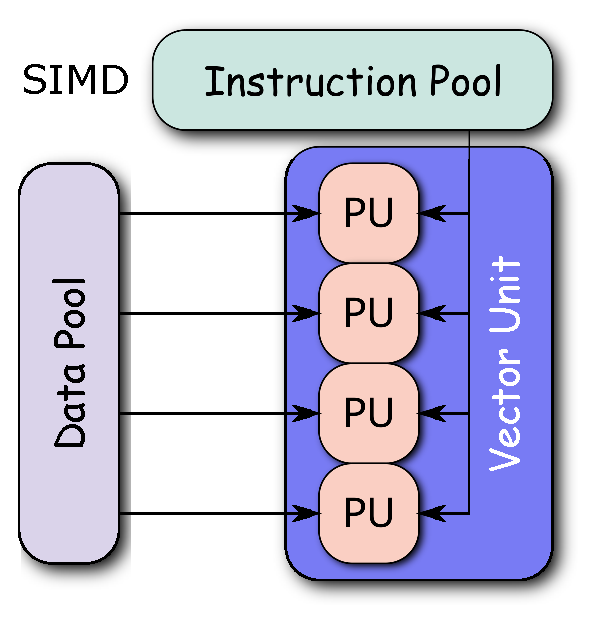
\includegraphics[width=0.5\textwidth]{./figures/SIMD2.eps}
	\caption{Vector processing units \cite{SIMDWiki}}
	\label{fig:simdUnits}
\end{figure}

Modern x86 processors from AMD and Intel provide different SIMD extensions named Streaming SIMD Extensions (SSE), Advanced Vector Extensions (AVX) with register size of 128-bits, Advanced Vector Extensions 2 (AVX2) with register size 256-bits and the latest AVX-512 with register size 512-bits. In this work, an AMD EPYC processor is used provides SSE, AVX and AVX2 instructions. Listing \ref{code:naiveAdd} shows vector addition implemented naively. Listing \ref{code:simdAdd} illustrates same operation using vector processing units. 

\begin{code}
	\captionof{listing}{Naive vector addition}
	\label{code:naiveAdd}
	\begin{minted}[frame=single]{c++}
	int16_t vec1[] = {1,2,3,4,5,6,7,8,9,10,11,12,13,14,15,16};
	int16_t vec2[] = {17,18,19,20,21,22,23,24,25,26,27,28,29,30
						,31,32};
	for(auto i = 0; i < 16; i++)
		vec1[i] = vec1[i] + vec2[i];
	\end{minted}
\end{code}

\begin{code}
	\captionof{listing}{SIMD Addition}
	\label{code:simdAdd}
	\begin{minted}[frame=single]{c++}
	int16_t vec1[] = {1,2,3,4,5,6,7,8,9,10,11,12,13,14,15,16};
	int16_t vec2[] = {17,18,19,20,21,22,23,24,25,26,27,28,29,30
					,31,32};
	
	__m256i reg1 = _mm256_load_si256 ((__m256i*)vec1);
	__m256i reg2 = _mm256_load_si256 ((__m256i*)vec2);
	reg2 = _mm256_add_epi16 (reg1, reg2);
	_mm256_store_si256 ((__m256i*) vec1, reg1);
	
	\end{minted}
\end{code}

\subsection{Recursive function calling mechanism}
Most of the encoder and decoder implementations are implemented through recursion. Recursive function is a function which calls itself. It is a powerful tool in computer science which can be used for solving many interesting problems \cite{CLRS}. However when it comes to performance, recursive problems solving fall behind algorithms which use loops to solve the same problem. Every time a recursive function is called, a new stack frame is allocated, local data is pushed to call stack and execution must branch to the beginning of function. Branching and pushing data to a call stack are expensive operations. In case of polar codes, both encoding and decoding are implemented as recursive functions. To reduce the latency of FEC chain encoding/decoding implementations are unrolled to avoid recursions. For the encoder, unrolling is carried out by manually implementing multiple inline functions. In decoder implementation unrolling is carried out by using template concept of C++. Although unrolling increases code size, for the application in hand latency is of at most importance than code size. Unrolling of the encoder and decoder implementations significantly improved the latency of FEC chain. Listing \ref{code:recursiveImpl} shows recursive implementation of factorial calculation. Listing \ref{code:unrolledImpl} illustrates same operation implemented with unrolled implementation. 

\begin{code}
	\captionof{listing}{Recursive implementation}
	\label{code:recursiveImpl}
	\begin{minted}[frame=single]{c++}
	int fact(int n) {
		if(n > 1)
		return n * factorial(n - 1);
		else
		return 1;
	}
	\end{minted}
\end{code}

\begin{code}
	\captionof{listing}{Unrolled implementation}
	\label{code:unrolledImpl}
	\begin{minted}[frame=single]{c++}
	template <unsigned Nv>
	inline int fact() {
		return Nv * fact<Nv - 1>();
	}
	
	template <>
	inline int fact<0>() {
		return 1;
	}	
	\end{minted}
\end{code} % Background about polar codes and their usage in 5G.
        \chapter{Encoding FEC Chain} \label{chap:encoder}

% In this document explain all the things which I have done until the midterm presentation.
% All the details, Optimization techniques I have employed.
% Following text might be useful for writing the text.
% Also my midterm presentations/office presentations will be really useful for writing this part.  
% Reference paper for explaining the different components of the this FEC chain "Design of Polar codes for 5G NR radio"

%Work I have done Until now.
%
%Optimizations to the original implementations until now.
%Generic optimizations
%- Using optimization primitives such as likely and unlikely.
%- Aligning memory to 32 bytes so copying of data can be vectorized.
%Polar transform optimization	
%- Replace binary additions with xor. instead of addition and then modulus two.
%- division and multiplications by left and right shift operations.
%- Avoided copy operations in polarTransform operations.
%Optimization in getting reliability indices.
%- Avoided remove and erase operations which have huge overhead. Wrote a efficient mechanism(reduced the latency by 176 us).
%- Instead removing and erasing I mark the element as removed.
%- Since the reliability indexes won't change. I built a look up table in place of searching all (1024)indices reduced the latency by 40us
%- Avoided copying operations of interleaved indexes.
%- Unrolled the loop to reduce the jumps.
%Rate matching optimizations.
%- optimization in subblock interleaving, Rewrote the logic to avoid E number of division and modulus operations.
%- Unrolled the for loops in subblock inteleaving method.
%- Implemented optimal version of bit selection, Avoided E number of modulus operations which are very costly.
%- Again optimization primitives for helping the branch predictor.
%
%
%Fast version of Encoding API's.
%In the original implementation of the polar encoding each of the bit is treated as 32 bit integer. This is highly inefficient
%when the goal is to process multiple bits at time. With each bit considered as 32 bit integer SIMD instructions won't provide
%any performance improvement. Reason is SIMD instruction can process multiple bits at time. avx2 instructions 256bits at a time.
%if we have 32 bits to represent a single bit. we can process only 8 bits at time. Which doesn't significantly improve the
%performance. To avoid this disadvantage and make use of SIMD capability. each 64 bit integer is considered as 64 bits of data.
%so one avx2 instruction can process 256 data bits in a single instruction.
%- Built a look up table to avoid last eight stages of polar encoding instead of traversing till end of tree.
%- Implemented SIMD instruction based encoding. Encoding happens within 0.6 us for N = 512.
%- Implemented optimal version of CRC calculation which can calculate CRC for PDCCH chain within 0.8 us. Original implementation was taking 7 us.
%- Implemented a bit interleaver which can deal with this format of data.

In this section, complete polar encoding FEC chain used in 5G is explained. Methods used for code profiling and latency measurement are presented. After figuring out the latency contributors code optimization/algorithm optimizations employed during the FEC chain development are presented and then presents how SIMD feature of the modern processors is exploited to obtain the low latency for PBCH and PDCCH FEC chains and frozen set selection algorithm improvement with the aid of look up table, finally presents the encoding process as traversal of a binary tree and how the encoding latency can be improved by pruning the tree hence avoiding the tree traversal instead using a lookup table to obtain the encoded result.

In 5G framework, Polar codes are used in downlink to encode downlink control information (DCI) over physical downlink control channel (PDCCH) and for payload in physical broadcast channel (PBCH). In uplink, to encode uplink control information (UCI) over the physical uplink control channel (PUCCH) and the physical uplink shared channel (PUSCH). In this work, notations introduced in 3GPP technical specification\cite{3gpp.38.212} are used.

The figure ~\ref{fig:5g_fec_chain} represents the complete polar FEC chain for PBCH and PDCCH in downlink. Let's look at each of the components briefly to understand the FEC chain. In general $A$ bits have to be transmitted over a code of length $E$ code bits. $L$ CRC bits are added to the information bits, resulting in  $K = (A + L)$ bits. These $K$ bits are passed through an interleaver. Interleaved bits are concatenated with a parity bits and assigned to information set to obtain a vector $\boldsymbol{u}$. Encoding is done with a mother code with parameters $(N,K)$, with $N = 2_{n}$. Encoding is performed $\boldsymbol{d = uG_{N}}$ the generator matrix $\boldsymbol{G_{N} = G^{\otimes n}}$ obtained by $n^{th}$ kronecker product of Arikan matrix. Encoded codeword $\boldsymbol{d}$ passed through a subblock interleaver which divides the codeword in to blocks of 32 bits and performs interleaving between them according to 32 integers (interleaving pattern is nothing but a bit reversal of bit position) shown in figure. \textbf{add picture of bit reversal operation}. After subblock interleaving is completed rate matching is carried out. To map $N$ to $E$ bits. Rate matching can repetition, puncturing or shortening. This decision is taken based on the value of $E$, $N$ and $K$. Finally to improve the error correction performance channel interleaving is done. This section of the report presents  implementation details of each of these operations in an algorithmic level with small code snippets whenever necessary. Analyzes latency introduced by different sections of FEC chain and also presents the algorithmic and platform specific optimizations.

\begin{figure}[h]
	\centering
	\includegraphics[width=0.7\textwidth]{./figures/5GFECChain.pdf}
	\caption{Polar Encoding FEC chain for PDCCH/PBCH}
	\label{fig:5g_fec_chain}
\end{figure}

\section{Data packing and Unpacking Operations} \label{dataPackUnpack}
Typically in software implementations, for clarity and ease implementation each bit of information is represented with 32-bit or 64-bit integers. Due to the presence of only one bit of information in each integer if want to encode/decode 1024 bits, then 1024 integers are involved in encoding/decoding process. However this isn't the case in hardware implementations since each bit can be processes in Harware Description languages (HDL). Representing each one bit of information using 32/64-bit integer has following disadvantages. 

\begin{description}[font=$\bullet$~\normalfont]
	\item Increased memory footprint: If one decides to represent each bit using 64-bit integer for 1024 bits of information 64*1024 bits memory needs to allocated which equivalent to 8 kilobytes. Allocating and initializing this memory can introduce significant latency.
	\item Results in more cache misses: If more memory is allocated then more data needs to accessed from DRAM which can result in significant number of cache misses.
	\item Serializes encoding/decoding: General purpose processor's have a data path width of 64-bit. If each bit is represented using 64-bit integer we are not using capability of processing 64 bits simultaneously instead each bit is processed sequentially. This can make encoding/decoding sequential although processor is capable of processing multiple bits in parallel.
\end{description}

To avoid these disadvantages and to enable data parallelism, this implementation of encoder tries to pack the multiple information bits to one integer. Although packing information bits to single integer has advantages, for some operations such as bit wise interleaving accessing each bit efficiently is very important. To exploit the advantages of bit packing as well as the advantages of each bit as integer, it is necessary to convert between the two. This is where the power of SIMD instructions in modern processors come to rescue. These processors come with special hardware instructions which help to efficiently pack and unpack data. Information bits are used in packed format when data parallelism needs to exploited and in unpacked format when certain operations require bits to accessed individually. These pack/unpack instructions are very efficient with low latency.

Some examples of these instructions are:
\begin{lstlisting}
	int _mm_movemask_pi8(__m64 a);
	int _mm_movemask_epi8(__m128i a);
	__m256i _mm256_unpackhi_epi8(__m256i a, __m256i b);
	/** many more **/
\end{lstlisting}

\TODO{May be give examples code snippet which packs and unpacks bits in an efficient manner.}

\TODO{cite to agner fog optimization manuals. \cite{AgnerFog} , \cite{DeltaFunction}}

\section{CRC calculation}
%Explain why CRC attachment is considered in whole FEC chain, how it is useful for decoding polar codes. Explain algorithmic complexity of CRC calculation, How much time it was taking, How the optimization is carried out to reduce the CRC calculation time.
As shown in the figure \ref{fig:5g_fec_chain} L-bit CRC is calculated for $A$ information bits and attached as part of message. Number of CRC bits (L) varies for different physical channels. In downlink, for payload of PBCH/PDCCH 24-bit CRC is used. Uplink Control Information (UCI) uses 6-bit or 11-bit CRC based on the value of $A$. For $12 \leq A \leq 19$ and $A \geq 20$ 6-bit CRC and 11-bit CRC are used respectively. Polynomials use for different CRC values is shown below \cite{3gpp.38.212}.

\begin{equation} \label{crc_polynomial6}
g_{6}(x) = x^{6} + x^{4} + 1
\end{equation}
\begin{equation} \label{crc_polynomial11}
g_{11}(x) = x^{11} + x^{10} + x^{9} + x^{5} + 1
\end{equation}
\begin{equation} \label{crc_polynomial24}
g_{24}(x) = x^{24} + x^{23} + x^{21} + x^{20} + x^{17} + x^{13} + x^{12} + x^{8} + x^{4} + x^{2} + x + 1
\end{equation}

Information bits concatenated with CRC increases the error correction performance of polar codes significantly. CRC is be used for selecting the correct code word out of potential candidates when employing a list-decoding algorithm. With CRC aided decoding, polar codes performance is very close maximum likelihood decoding. To reduce the latency of encoding FEC chain CRC needs to calculated very efficiently. One of the naive implementation of CRC calculation is, by using shift register method, which calculates CRC sequentially for one bit at a time as given in \cite{naiveCRCCalculation}. As explained in the section \ref{dataPackUnpack}, it is very inefficient to process bits sequentially. Instead one can calculate the CRC blockwise with the help of lookup table. In otherwords, divide the data into blocks of $B$-bits, read the corresponding CRC value from lookup table and combine individual CRC's of blocks in an predefined way to create a CRC for complete data. Algorithm in \cite{Sarwate:1988:CCR:63030.63037} is adopted to calculate CRC24 using lookup table based approach. Data bits are divided into blocks of 8-bits and packed into 8 bit integers. CRC value corresponding to 8-bit integer is read from lookup table and combined with CRC of subsequent 8-bit integer, this process continues until CRC of data bits is completed. If the number of data bits are not multiple of 8 then zero's are appended at MSB position.  Table \ref{tab:crcLatencyTable} presents the latency values of naive and optimized  CRC calculation methods for payload of 41-bits on AMD EPYC processor running at 1.6 GHz with Turbo disabled. There is significant improvement in the optimized method compared to naive implementation.

\begin{table}[h!]
	\begin{center}
		\caption{CRC24 calculation latency comparison}
		\label{tab:crcLatencyTable}
		\begin{tabular}{c|c|c} % <-- Alignments: 1st column left, 2nd middle and 3rd right, with vertical lines in between
			\textbf{ } & Naive & Optimized \\
			\hline
			Latency ($\mu$s) & $9.3$ & $0.016$\\
		\end{tabular}
	\end{center}
\end{table}

\section{Input Bit Interleaver}
\TODO{Any optimization carried out in here, need to be explained clearly, Why this input bit interleaver is necessary. How much time this function takes.}

\section{Polar code construction}
\TODO{Here explain the algorithm how frozen/information/parity indices are selected. With an algorithm and flow chart which makes very clear/easy to understand the algorithm. Explain the effect of puncturing and shortening on the bit reliability. May be mode should be selected, either as puncturing/shortening at constructor. And corresponding operations are performed accordingly. Give also the details about information bit insertion reliable locations. Explain the effect of puncturing and shortening on the reliability of bit channels.}




\section{Polar Encoding}
Explain how the matrix multiplication is transformed into recursive formulation. Represent the encoding procedure as traversing through binary tree. How the parallelism of SIMD processor is exploited speed up the encoding process. Explain the employed tree pruning method.

\section{Results Comparison}



 % Contains the details of encoding FEC chain.
        %%%%%%%%%%%%%%%%%%%%%%%%%%%%%%%%%%%%%%%%%%%%%%%
\chapter{Decoding FEC Chain} \label{chap:DecodingChain}
%%%%%%%%%%%%%%%%%%%%%%%%%%%%%%%%%%%%%%%%%%%%%%%
In this chapter, implementation and optimization details of 5G polar decoding FEC are presented including challenges faced while achieving low latency decoding. In FEC chain, decoder is the critical part due to inherent sequential nature of polar decoding. $n^{th}$ bit is decoded by using all the previously decoded bits, hence $n^{th}$ bit depends on $0$ to $n-1$ bits. Due to sequential decoding process, significant latency is introduced by the decoder. This section presents the optimization techniques employed to improve the latency, which include both algorithmic and platform specific optimizations. Each these techniques are explained in the respective sections where these are employed. In this work, FEC chain considered is part of the base station, therefore uplink control information is decoded at receiver. PUCCH (Physical uplink control channel) and PUSCH (Physical uplink shared channel) contain polar encoded information. Received signal after demodulation is quantized to 16-bit LLR (log likelihood ratio) values. Decoding is performed with LLR (Log likelihood ratio) values rather than probabilistic likelihoods due to their numerical stability and low computational complexity. Receiver side FEC chain is a reverse of the operations performed at transmitter. Figure ~\ref{fig:5grx_fec_chain} shows the receiver side polar decoding FEC chain.

\begin{figure}[]
	\centering
	\includegraphics[width=0.7\textwidth]{./figures/receiverFECChain.pdf}
	\caption{Polar decoding FEC chain for PUCCH/PUSCH}
	\label{fig:5grx_fec_chain}
\end{figure}

%$\mathtt{Yadhu}$
%\NOTE{Decoding is of serial nature, has lot of latency. Polar decoding chain necessity. PUCCH and PUSCH, parameters of both the channels.}
%%	Explain all the decoding Optimizations I have done, In this document.
%% 	Explain of the latency without optimization.

\section{Decoding algorithms}
The basic decoding algorithm successive cancellation (SC) is developed by the Arikan in his seminal work on polar codes \cite{Arikan}. It achieves the symmetrical capacity of binary memoryless channel through sequential decoding when block length is very large. However due to the sequential nature significant latency is introduced by decoding algorithm. Latest 5G standard specifies transmission time interval (TTI) of $125 \mu s$ \TODO{cite the doc}, within this duration scheduling and encoding/decoding must be done. Therefore it is very important to efficiently perform FEC chain operations. This work concentrates on implementing the polar encoding/decoding in software and studies the feasibility of satisfying the strict latency requirements of 5G. Decoding through SC algorithm can be represented as binary tree, decoding process is nothing but traversing through a tree sequentially. Significant research work is done both in academia and industry to improve decoding latency of the SC algorithm. Major improvement to SC which significantly reduced the decoding latency is identifying special kind nodes in a tree which allow immediate decoding of multiple bits without requiring full tree traversal. Algorithms presented in \cite{SSC} and \cite{fastSSC} present such improvements, which identify special nodes or in other words component codes such as \textit{Rate-0}, \textit{Rate-1}, \textit{RPC} and \textit{SPC} nodes, \textit{RPC} and \textit{SPC} mean repetition and single parity check code respectively. Identification of special nodes requires finding particular patterns the frozen bit locations in the constructed polar code. To gain full advantages of Fast-SSC (Fast Simplified Successive Cancellation) algorithm, special nodes must be identified efficiently. In this work, 5G RX FEC chain with fast-SSC algorithm implemented/optimized in software and feasibility of achieving desired latency( $< 50\mu s$) is analyzed.
%Following sections present how processor specific features are exploited to efficiently identify


\section{Decoding chain}
The figure ~\ref{fig:5grx_fec_chain} shows the complete receiver side FEC chain. It is almost a inverse operations of encoding FEC chain except few differences related to PUCCH and PDSCH which contain parity check bits ($ n_{PC} $). The decoding FEC chain receives UCI(Uplink Control Information) in the form of 16-bit quantized $ E $ LLR values. Before passing LLR values to decoder inverse operations of the steps which were carried out aftermath of encoding, which are channel deinterleaving, inverse rate matching and subblock deinterleaving. These steps grouped by a pink rectangle in the figure, after these steps polar code construction is performed using same optimized method as presented in the previous chapter. Polar code construction procedure outputs the information bit positions, from which frozen pattern can be obtained. Next step in the FEC chain is polar decoding, $ N $ LLR values and frozen pattern is passed to polar decoder, which outputs the decoded bits. Polar construction and decoding blocks are colored green the FEC chain figure. Using information bit positions obtained in the polar construction procedure $ K + n_{PC} + L $ bits are extracted from $ N $ decoded bits. $ K + n_{PC} + L $ bits contain $ n_{PC} $ parity bits, extracting these bits requires identifying the row of minimum weight from the generator matrix of polar code. Finally input deinterleaving is applied on the remaining $ K +  L $ bits to obtain concatenated information and CRC bits. Blocks representing Extracting parity bits and input bit deinterleaver are grouped with blue rectangle. In this section, we presented briefly the functionalities carried out by different blocks of the decoding FEC chain. Next we will analyze the latency contributions of each those operations and come up with optimizations both algorithmic and platform specific to reduce latency.

\section{Channel deinterlever}
The first operation after receiving the LLR values is channel deinterleaving, This is the exact inverse of the interleaving operation done at the transmitter. Channel interleaving is performed to make transmission robust against burst errors. Authors of \cite{3gpp.TSG-RAN_WG1} analyze the error correction performance of polar codes for different channel conditions and constellations. It is found that error correction performance significantly deteriorates for constellations 16-QAM onwards. Channel interleaving wasn't done for downlink PBCH/PDCCH since the constellation was QPSK, however in case of PUCCH/PUSCH higher constellations are used hence channel interleaving is necessary. In 5G standard  isosceles right triangle interleaver is adopted. Deinterleaving is carried out by writing LLR values to columns of triangular structure and reading LLR values in rows. Interleaver design is proposed by Qualcomm \cite{3gpp.TSG-RAN_WG1}.

Vector processing instructions cannot be used for the implementation of interleaver due irregular and non uniform memory access, therefore interleaver just plain functional implementation. One optimization technique was to avoid new memory allocation and using already allocated memory. This avoids the overhead of dynamic memory allocation and initialization. Channel deinterleaving is one of significant contributor to latency in polar decoding FEC chain, since each of the LLR values need to processed sequentially.

\section{Inverse rate matching}
Inverse rate matching step maps the $E$ LLR values to mother code block size $ N $. Rate matching step has three modes puncturing, shortening and repetition. Mode is selected based on rate matcher output size ($E$) and mother code size($ N $). If $E > N$ then repetition performed, otherwise either puncturing and shortening is done. If $ \frac{K}{E} > \frac{7}{16} $ shortening else puncturing is performed. Major optimization in inverse rate matching are utilizing SIMD capability for soft combining when $ E>N $ and performing block wise copying. \NOTE{Does it makes sense to explain criteria why puncturing or shortening is selected}
%
%to and avoiding a copying operations when the mode is shortening or puncturing instead using a pointer manipulation to select
%Software optimization in inverse rate matching is performed by Empirically it is observed that shi  type of rate matching is selected based on code rate.
%
\section{Sub-block de-interleaver}


\section{Decoder optimization}

\subsection{Identifying component codes}
How different kind of sub code types are identified efficiently using with bit packed frozen bits.

\subsection{Decoding Rate-0 code}

\subsection{Decoding Rate-1 code}

\subsection{Decoding RPC code}

\subsection{Decoding SPC code}

\section{Extract Info Bits}
Means select information bits from the reliable positions.

\section{Extract parity check bits}


          % Include ... / Einbinden des Kapitels ...
        \chapter{Conclusion and Outlook} \label{chap:conclusion}
The objective of this work is to study the feasibility of developing polar FEC chain of 5G in software on general-purpose-processor while satisfying stringent latency requirements. In other words, all the components of encoder and decoder FEC chain are developed on general purpose AMD EPYC processor. The software satisfies latency constraint of less than 50$\mu$s. In the first part of the thesis, we provide necessary background about polar encoding/decoding and computer architecture. In the second part, we develop encoding and decoding FEC chains and optimize them to satisfy the necessary latency constraints. \newline

To begin with, we provided necessary mathematical background about polar code construction, polar encoding, and decoding. Including different polar decoding algorithms. To understand FEC chain development in software it is necessary to know the basics of modern computer architecture. Computer architecture section talks about pipelining, cache memory and vector processing units in modern general purpose processors. \newline

In the next chapter, we talk about the details of polar encoding FEC chain. In this chapter, we analyze the different components of the FEC chain to identify latency contributors. Each of these latency contributors is further studied to reformulate the algorithm to avoid costly operations. Algorithms are reformulated to fit into specialized functional units of modern processors such as vector processing units. Vector processing units allow data parallelism in addition to supporting very fast mathematical computations. The encoding,  major latency contributors were polar code construction, CRC calculation, encoding, and rate matching. A wide range of optimization techniques is employed to reduce the latency both algorithmic and platform specific. Namely, reducing algorithm complexity, using lookup tables, compiler hints for better instruction scheduling, vector processing instructions for data parallelism and avoiding superfluous copy operations et cetera. Optimizations reduced the worst-case latency of the encoding FEC chain from $451 \mu$s to $40\mu$s which is more than 10x reduction in latency. \newline

For the decoding FEC chain again same steps as encoding chain are followed to identify the latency contributors. Major contributors in decoding FEC chain were channel deinterleaver, subblock deinterlever, polar decoder, parity bit extractor, and CRC calculation. Decoding FEC chain extensively uses SIMD, bit count, cache prefetching instructions to reduce latency. Subblock deinterleaving operation is divided into three primitive small operations which are implemented efficiently with $\mathtt{permute}$ and $\mathtt{blend}$ vector instructions. The polar decoder is optimized by implementing XOR, CN, VN, bit combination and frozen pattern identification operations using vector processing instructions. Parity bit extractor optimized by avoiding expensive remove and erase operations instead uses modified algorithm marking indexes and dynamically calculating hamming weights of generator matrix rows. Finally, for CRC calculation an algorithm based on lookup table is developed based on \cite{Sarwate:1988:CCR:63030.63037} which processes block of data bits to calculate CRC. These optimizations significantly reduced the latency of decoding FEC chain from $391 \mu$s to $40\mu$s almost a 10x reduction in latency. \newline

As an outlook, for the above stated decoding FEC chain, decoder is developed with \emph{fast-SSC} algorithm. This algorithm has much lower error correction performance than similar block-length LDPC and Turbo counterparts. As part of this work, \emph{CRC-Aided Successive Cancellation List} (\emph{CA-SCL})\cite{SCL} decoding algorithm is also implemented, however, it is not optimized for software. \emph{CA-SCL} ideally suits very low SNR scenarios such as mmWave communication. It has approximately $1.5dB$ gain over \emph{fast-SSC} algorithm for $N=2048$ and list size $L = 8$. Ideal continuation of this work would be to extend the decoding chain by incorporating \emph{CA-SCL} algorithm to the FEC chain. It would be interesting to see the latency values of this algorithm, which has expensive \emph{sort} and \emph{copying} operations.   % Include conclusion/summary / Einbinden des Kapitels Zusammenfassung/Ausblick
        
        \cleardoubleemptypage

% ########################################
% Appendix / Anhang:
% ########################################

% roman page numbering, starting with page number 1 (capitals)/ roemische Seitennummerierung beginnend mit Seite 1 (gross)
    \appendix
    \setcounter{page}{1}
    \pagenumbering{Roman}

        % Use IEEE DIN 1505 style for bibliography / Literaturverzeichnisses
        \bibliographystyle{IEEEtr}
        \nocite{*}              % Include all references without checking / Alle References immer aufführen
        \bibliography{literature}

\end{document}

%
% EOF!
%